% vim: set fecn=utf8 ft=latex encoding=utf8
% -*- mode: latex; coding: UTF-8; -*-

\newif\ifdraft
\drafttrue

%%% blobtree.tex

\ifdraft
	\documentclass[conference]{acmsiggraph}
	\def\baselinestrech{1}
	\setlength{\marginparwidth}{2cm}
	\newcommand{\Title}{Implementing the Blob Tree | Draft}
\else
	\documentclass[conference]{acmsiggraph}
	\newcommand{\Title}{Implementing the Blob Tree}
\fi

\newcommand{\Author}{Evan T. C. Wilde}
\newcommand{\Email}{etcwilde@uvic.ca}
\newcommand{\Subject}{Implementing the Blob Tree}
\newcommand{\Keywords}{implicit surface, iso-surface, blobs, blobbies, blobtree}

\synctex=1

\usepackage{xspace}
\usepackage{amssymb}
\usepackage{amsmath}
\usepackage{breqn}
\usepackage{svg}

\hypersetup{pdftitle={\Title},
        pdfauthor={\Author},
        pdfkeywords={\Keywords},
        pdfsubject={\Subject},
        urlcolor=blue,citecolor=black}


\def\BibTeX{{\rm B\kern-.05em{\sc i\kern-.025em b}\kern-.08em
    T\kern-.1667em\lower.7ex\hbox{E}\kern-.125emX}}

\TOGonlineid{000000000}
\TOGvolume{0}
\TOGnumber{0}

\ifdraft
	\usepackage[colorinlistoftodos]{todonotes}
		\newcommand{\evan}[1]{{\color{cyan}\emph{Evan Says:
		#1}}\xspace}
		\newcommand{\evanTodo}[1]{{\color{blue}\emph{Evan Todo:
		#1}}\xspace}
\else
	\usepackage[disable]{todonotes}
	\newcommand{\evan}[1]{}
	\newcommand{\evanTodo}[1]{}
\fi

\newcommand{\fff}{field falloff function}


%%% Local Variables:
%%% mode: latex
%%% TeX-master: "marching-triangles"
%%% End:


\title{\Title}
\author{
	\Author \\
	University of Victoria\\
\Email}
\pdfauthor{\Author}
\keywords{\Keywords}

\begin{document}

\teaser{
	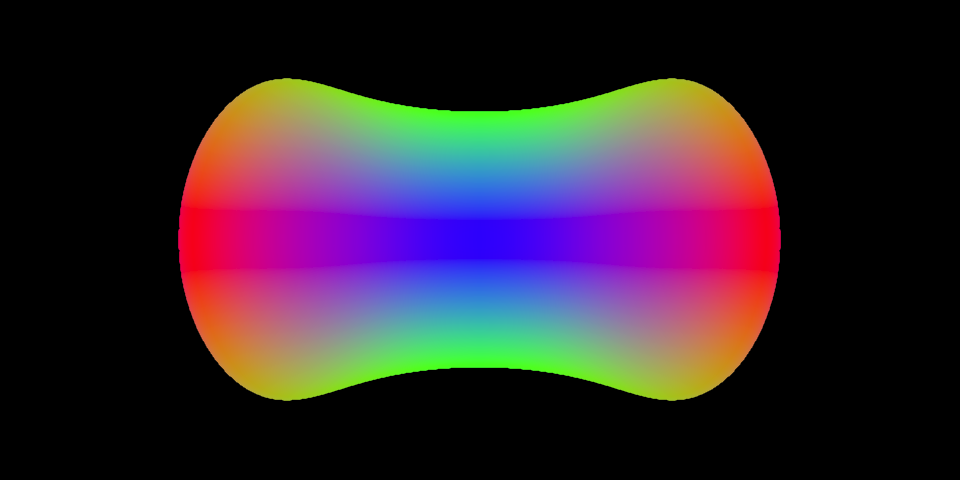
\includegraphics[height=1.5in] {images/blend.png}
	\caption{Blended Blobs}
}

\maketitle

\begin{abstract}
	Implicit surfaces are a mathematical representation of geometric
	information; storing complex geometric information with minimal memory
	requirements. Blobs are a form of implicit object defined by a central
	origin point, a \fff, and an iso value. The surface is defined at
	radius $r$ when the \fff evaluated on $r$ is equal to the iso value.

	A blob tree is used to build complex geometry from simpler
	primitives. Intelligent construction of the blob-tree is critical for
	fast evaluation of the implicit object represented in the tree, whether
	that be for ray-tracing or polygonization.

\end{abstract}

\keywordlist

\copyrightspace

\section{Introduction}

Implicit surfaces are a mathematical representation of geometric information;
storing complex geometric information with minimal memory requirements.
Implicit surfaces can be represented with implicit equations or as blobs. The
implicit equation form uses algebraic formulas to define shapes, for example a
sphere is represented by the equations $x^2 + y^2 + z^2 = R^2$, where $R$ is
the radius of the sphere. A more complex shape defined by an implicit equation
is a jack,

\begin{dmath*}
\left({1 \over ({x^2 \over 9} +  4y^2 + 4z^2)^4} +
{1 \over ({y^2 \over 9} +  4x^2 + 4z^2)^4} +
{1 \over (({4x \over 3} - 4)^2 + {16y^2 \over 9} +  {16z^2 \over 9})^4} +
{1 \over (({4x \over 3} + 4)^2 + {16y^2 \over 9} +  {16z^2 \over 9})^4} +
{1 \over (({4y \over 3} - 4)^2 + {16x^2 \over 9} +  {16z^2 \over 9})^4} +
{1 \over (({4y \over 3} + 4)^2 + {16x^2 \over 9} +  {16z^2 \over 9})^4}\right)^ {-
	{1\over 4}} - 1
\end{dmath*}
\cite{Bloomenthal1994}

Due to the complexity of the algebraic equations for complex models, a model
was proposed which constructed complex geometry from simpler primitives using
the operations union, different, and intersect.

A separate branch of implicit surfaces is the blob, or the blobby molecule
defined by Jim Blinn \evan{cite} for observing the behaviour of electron
density fields. Blobs are defined in three parts: a center point, a filter
field falloff function, and an iso value. The central point is the point around
which the blob exists. The filter field falloff function is a function where at
the center point is at its highest value, and at some maximum radius $R$ is 0.
The iso value specifies the value of the evaluated filter field falloff
function to define surface. That is, at some distance $r$, if the filter field
falloff function evaluates to the iso value, then the surface is defined at the
radius $r$.

Brian Wyvill proposed a new structure combining the power of CSG trees and
blobs into one structure, the blob tree. Blob trees are a data structure for
containing and evaluating geometric information stored as blobs. A blob tree
represents the complex geometry in a hierarchy where the root node is the
intended shape and the leaf nodes are the primitive objects. The interior nodes
are the various operations that can be performed on the primitives and simpler
objects. These operations can be combined in various ways to design more
complex objects.

In this paper, we explore the implementation details of a simple blob tree
structure and the various additions that can be implemented to increase the
performance and robustness of the tree for various uses.

The implementation of the tree is available on github\evan{Implicit system
GitHub Link}, with the accommodating implementation of the raytracer used to
generate the images in the papers\evan{Github raytracer link}


\section{Related Work}
Jim Blinn used blobs, or blobby molecules as a way of representing electron
density fields\cite{Blinn}. Using blobs as a way of modeling has interesting
advantages to simply working with algebraic implicit surfaces. Brian Wyvill
worked to combine the power of CSG trees and blending of blobs to create a new
implicit system, the blob tree. Blob trees are capable of all the basic CSG
operations, such as union, intersect, difference, and warp, but also include
the blend operation which will blend the blobs together when they get within a
certain distance of each other. That is, the blobs can effect the shape of the
blobs surrounding it.

\section{Implementation Details}
In this section, we describe the methods of implementing the blob tree, and why
we made a given decision.


\subsection{Finding Surface}
Finding the point where the surface exists proves to be challenging, as the
\fff\ is not necessarily invertible. To find the surface, a numerical
root-finding method is required. I used the secant method, described as
follows:
\begin{equation}
x_i = x_{i-1} - f(x_{i-1}) \times {x_{i-1} - x_{i-2} \over f(x_{i-1}) -
f(x_{i-2})}
\label{eq:SecantMethod}
\end{equation}

The secant method was chosen due to the relative speed of convergence, not
requiring bracketing, and not requiring derivations. The bisection method
guarantees convergence and does not require differentiation; however, it
requires a bracket to be placed on the surface, and has linear convergence. The
Newton-Raphson method is an open method that has order $n^2$ convergence, but
requires derivations and cannot guarantee convergence. The secant method is
another open method that has order $n^{1.618}$ convergence and does not require
derivations, but cannot guarantee convergence. Furthermore, as an open interval
method, the initial point must be close enough to the shape that the \fff\ has
an effect.

For the purpose of polygonization, it is possible to use the centre point of a
given primitive, which will be at the centre of the field function. In most
cases, given the Geoff \fff, the secant method will converge within 6
iterations. For this purpose, no extra measures are necessary to ensure
convergence.

\begin{figure}[htb]
	\centering
	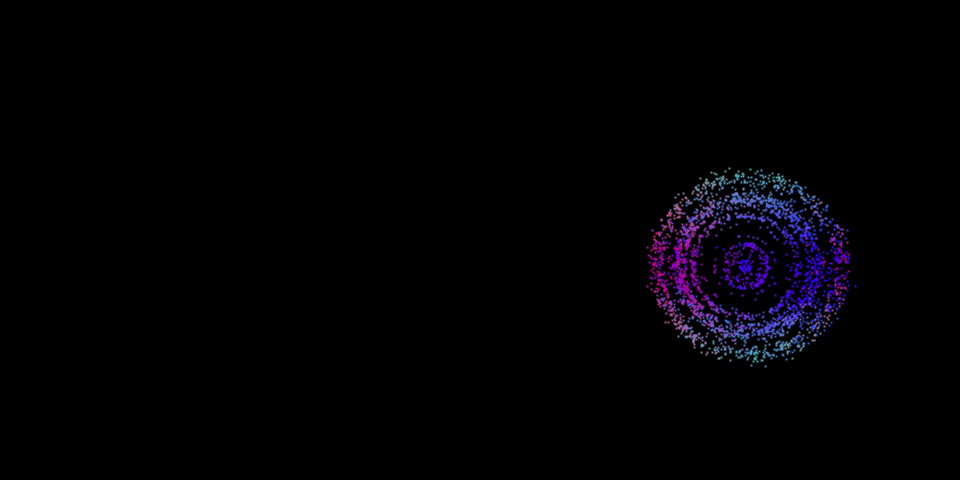
\includegraphics[height=1.5in] {images/sphere_no_bvh.png}
	\caption{Ray-traced blob without bvh}
	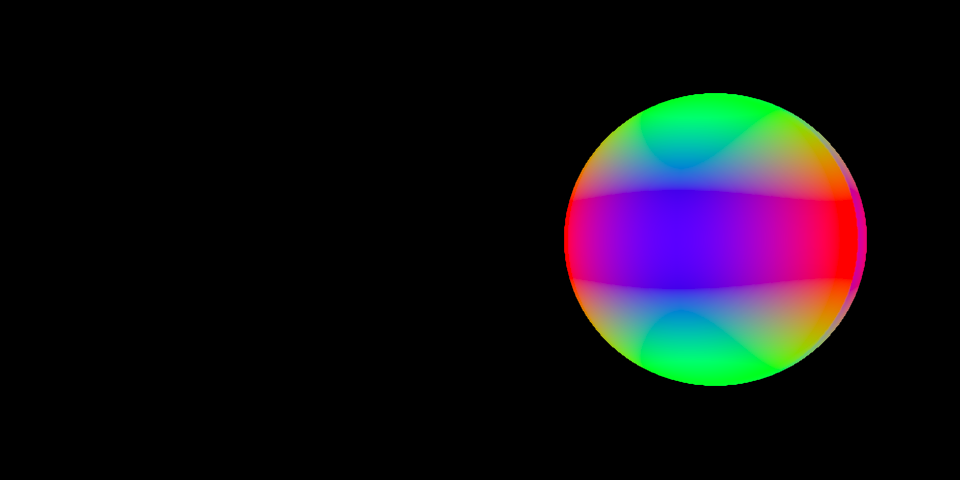
\includegraphics[height=1.5in] {images/sphere_bvh.png}
	\caption{Ray-traced blob with bvh}
\end{figure}

For the purpose of raytracing, in most cases the rays being sent toward the
object are beyond the maximum radius of the \fff\ and the secant method is
unable to converge. For this, we implemented a simple bounding volume
hierarchy, which is able to quickly determine which rays get close enough to
the surface that the \fff\ will have values different than zero.

\subsection{Primitives}
The current implementation has the spherical blob primitive. This is the
simplest primitive for blobs to represent. A spherical blob consists of a
centre point $center$, a filter field falloff function $f(r)$, and an iso value
$iso$ where the surface is defined.

The \fff we have implemented is the Geoff function: $r$ is the defined by the
distance from the central point, $R$ is the maximum effective distance of the
\fff.
\begin{equation}
f(r) = 1 - {4\over9} {r^6 \over R^6} + {17 \over 9} {r^4 \over R ^ 4} -
{22\over 9} {r^2 \over R^2}
\label{eq:GeoffFunction}
\end{equation}

In the blob tree, primitive objects are the simplest object and therefore are
always leaf nodes.

\textbf{Evaluating the field function}\\
Given $p$ and a sphere primitive, the field value is evaluated as:

\begin{equation}
F(p) = f(\lvert p - center \rvert)\\
\label{eq:FieldValue}
\end{equation}
\begin{equation}
E(p) = f(\lvert p - center \rvert) - iso
\label{eq:SurfaceEvaluate}
\end{equation}



In equation \ref{eq:FieldValue}, the result of the function must be compared with
the iso value to determine where the surface is. For this reason, it is helpful
to simply define another function \ref{eq:SurfaceEvaluate} which subtracts the
iso value from the evalutated field value. To distinguish the two functions I
call function \ref{eq:FieldValue} ``Field evaluation'', and function
\ref{eq:SurfaceEvaluate} ``Surface evaluation''.

Equation  \ref{eq:FieldValue} is called during the traversal of the tree. This
is useful for performing the various operations on the primitive objects.
Equation \ref{eq:SurfaceEvaluate} is used primarily for the purpose of root
finding, since the root-finding method will tend to zero rather than an
arbitrary value. Furthermore, the surface evaluation function
\ref{eq:SurfaceEvaluate} behaves more like the algebraic form of implicit
surfaces over the blob-form of implicit surfaces.


\textbf{Evaluating the normal}\\
Given $p$ and a sphere primitive, the normal is evaluated as:
$$ \overleftarrow{N}(p) = {p - center \over \lvert p - center \rvert}$$

\subsection{Transforms}
We implemented the three basic transforms: translation, rotation, and scaling.
The transform class simply takes any 3-dimensional homogeneous matrix, making
the implementation of the translation, rotation, and scaling operations
trivial. The use of an over-arching transform class simplifies.

\begin{figure}[htb]
	\centering
	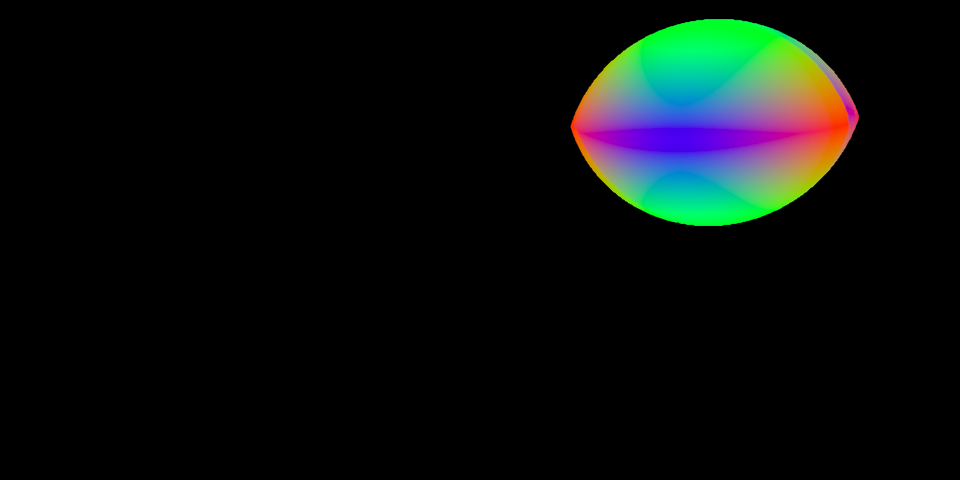
\includegraphics[height=1.5in]{images/intersect_rotate.png}
	\caption{Intersected Spheres Rotated then Translated}
\end{figure}

\subsection{Operations}
Blob-trees are able to perform various binary operations between two
sub-trees. Our implementation provides three of the five possible operations;
the blend, union, and intersect operations. The two remaining operations are
the warp, which is not a binary operation, but includes tapers and twisting,
and difference, allowing blobs to remove volume from another blob.

We describe the method of calculating the field value and normal vector for
each given operation.

The method for calculating the field values of the various operations is
described thoroughly in \textit{The BlobTree} \cite{Wyvill}.

\begin{enumerate}
	\item Primitive:\\
		$F(p)$\\
		$N(p) = {center - p \over | center - p |}$
	\item Blend:\\
		$F(L(o), p) + F(R(o), p)$\\
		$N( $

	\item Union:\\
		$max(F(L(o), p), F(R(o), p))$
	\item Intersect:\\
		$min(F(L(o), p), F(R(o), p))$
\end{enumerate}

The primitive does not contain any children, and therefore will simply
evaluate the field value with respect to the distance from the centre point.
Similarly for calculating the normal vector, the primitive has no children, so
the normal will be calculated as follows.

\subsection{Instancing}
By using instancing, we are able to minimize the memory usage by not
duplicating simpler geometry to build more complex geometry. As an example, a
union object can be made of a single primitive $p$, translated by some
distance. We get the effect of two separate primitive instances, but we only
use the memory of a single instance.

In implicit systems, instancing has further performance benefits as it
introduces the concept of local and world coordinates. An example of where this
is particularly useful is when scaling the sphere. It is a lot simpler to
perform a ray-sphere intersection than to perform the intersection test on a
ellipsoid. By mapping the ray into the local coordinate system, we are able to
leave the object as a sphere by bending the world and rays around it.

\subsection{Normal Data}
Normal is defined by the normalized weighted linear combination of the normal
vectors of the contributing component spheres, where the weights are defined by
the contribution to the iso-value of the corresponding component
sphere\cite{Wyvill}.

\subsection{Curvature}
We are looking for the principal curvatures at a given point on the surface.
The principal curvatures $k1$ and $k2$, define the curvature along the tangent
and bi-normal vectors to the given point. The method for finding the curvature
is described in section four of \textit{Curvature Formulas for Implicit
Surfaces} \cite{Goldman2005}. By using a cofactor approach, we can find the adjoint matrix to the
hessian, $H'$. 

$$
H'(F) =
\begin{bmatrix}
	F_{yy}F_{zz} - F_{yz}F_{zy} & F_{yz}F_{zx} - F_{yx}F_{zz} & F_{yx}F_{zy} - F_{yy}F_{zx} \\
	F_{xz}F_{zy} - F_{xy}F_{zz} & F_{xx}F_{zz} - F_{xz}F_{zx} & F_{xy}F_{zx} - F_{xx}F_{zy} \\
	F_{xy}F_{yz} - F_{xz}F_{yy} & F_{yx}F_{xz} - F_{xx}F_{yz} & F_{xx}F_{yy} - F_{xy}F_{yx}
\end{bmatrix}
$$
By performing the adjoint operation on $H'$, we can get the
hessian matrix $H$. Then we can use the mean $k_M$ and gaussian $k_G$
curvatures to find
the principal curvatures $k1$ and $k2$ with the formula:
$$k1, k2 = k_M \pm \sqrt{k^2_{M} - k_G}$$


$$k_M = {\nabla F * H'(F) * \nabla F^T \over |\nabla F|^4}$$

$$k_G = {\nabla F * H(F) * \nabla F^T - |\nabla F|^2 * H_{diagonal} \over 2 *
|\nabla F|^3}$$

I would like to investigate a method for finding curvature described in another
paper\cite{DeAraujo2004} to see which handles sharp-edges and discontinuities
better, and which method can be evaluated more quickly.

The method described by De Ara\'{u}jo uses the partial derivatives of the
normal vector in a single matrix, rather than computing multiple matrices.

$$
C=
\begin{bmatrix}
	{\partial N_x \over \partial x}&{\partial N_x \over \partial y}&{\partial N_x \over \partial z}\\
	{\partial N_y \over \partial x}&{\partial N_y \over \partial y}&{\partial N_y \over \partial z}\\
	{\partial N_z \over \partial x}&{\partial N_z \over \partial y}&{\partial N_z \over \partial z}
\end{bmatrix}
$$

The matrix C can be defined using the hessian matrix and the normal vector.

\subsection{Bounding Volume Hierarchies}
We implemented the bounding volume hierarchy (bvh) using axis-aligned bounding
boxes(AABB). We used this construction due to the simplicity and speed of the
intersection testing. From the use of AABB for rendering and collision
detection in video games, many optimized methods of intersection have been
developed\cite{Williams}.


\section{Findings}
In this section, we describe how the decisions made effected the resulting
speed and robustness of the blob tree.

\subsection{Bounding Volume Hierarchies}
We found that while the bvh greatly improved the rate of convergence of the
secant method, taking an average of four iterations with the bvh versus the
twenty iterations without, and increased the number of locations where it did
converge, we did not find that our naive approach had any effect on the overall
speed of the ray tracing program, which should have received the most benefit
from such a structure.

\subsection{Limitations}
By the description of the normal calculation, our implicit system is only
capable of working with primitive spheres.

\section{Future Work}
\subsection{BVH}
We would like to look into utilizing the bounding volume hierarchy to get more
performance from the system. While optimized methods were used for testing and
locating intersection points, we would like to use the bvh to determine when we
need to evaluate a branch of the subtree.

\subsection{Primitives}
Another area on extending the blob tree is implementing more primitive skeletal
objects, such as a: torus, cube, and line primitive. The implementation of the
normal calculation could remain the same, but the normal calculations for the
other primitives would either have to be sampled, as described in the Autodesk
paper, or specific methods for the desired shape could be implemented.

\subsection{Field falloff functions}
As of this time, we have implemented and worked with the Geoff function. Future
work could include observing the effects of other \fff s.

\bibliographystyle{acmsiggraph}
\bibliography{references}
\end{document}

